\begin{post}
	\postdata{Shine Your Light}{2011}{11}{23}{0}{3}{5}
	\begin{content}
Writing this post finally made me look up the song I have had in my head since Saturday. I could remember just few lines from it and I could not remember the rest or who it sings. Now I now, it was Roxette — Love Is All (Shine Your Light). And why I had this song in my head? Because of the light!

\begin{figure}[h]
\centering
\fbox{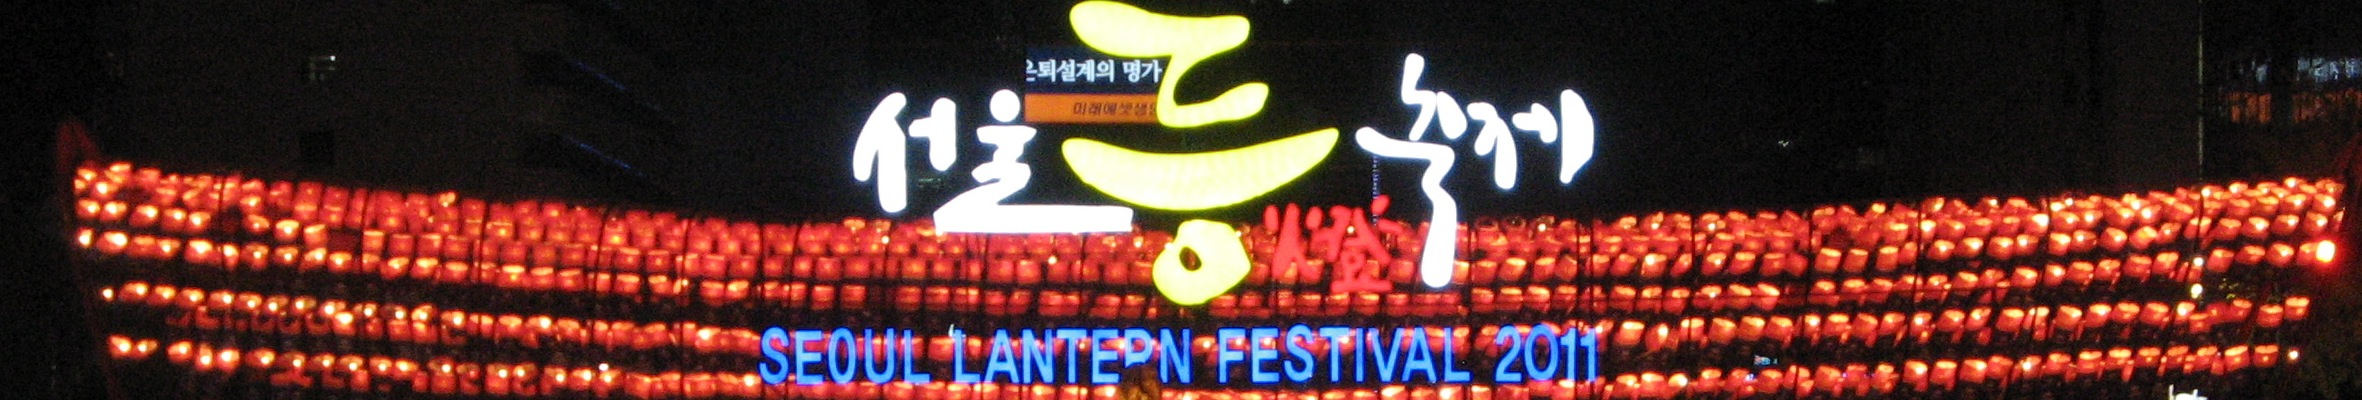
\includegraphics[width=1.0\textwidth]{photos/11/23/img_2060.jpg}}
\end{figure}

Until last Sunday, Seoul had hosted the traditional Lantern Festival on the Cheonggyecheon Stream in the City Hall area downtown Seoul. To let some more culture into our lifes, we have decided to go there. At first, it was Kate, Marc, André, Rik and me. Since Marc was meeting some friend earlier, it was just Kate, André, Rik and me. Well, and because Kate had some other things to do, it was just...I think you know now.

Upon arriving to City Hall, we have discovered three things. Firstly, there was a huge ``Occupy Seoul demonstration in front of the City Hall. For unknown reasons, these people were protesting against the FTA with the US, which is weird, because I thought that it was generally accepted very well. The second thing was the presence of riot police in the whole neighborhood — police buses, anti-riot vehicles and policemen in full body armor with shields, everything looked like there was going to be a huge fight. The third thing was my SD card, or rather its absence. As soon as I took out my camera, I realized that the card is still in my laptop, which gave me space for only two or three pictures in the internal memory. Fortunately André was there to save the day, so all the photos in this post are from him. Merci beaucoup!

Before coming to the festival we made a short detour to Lotteria for a Giant Double Burger set (912 Kcal of pure awesomeness) and then straight to the lanterns! Well, not that straight. Since it was the penultimate night, there was quite a queue that was twisting and turning between the barriers. Even though we managed to jump part of the queue by simply walking next to all the people (smart guys), eventually we reached the point where we had to re-join the queue and wait. And wait. And wait. In total, we waited for approx. 20 minutes, which was quite uncomfortable, since it was around 0°C.

\begin{wrapfigure}{L}{0.5\textwidth}
\vspace{-12pt}\centering\fbox{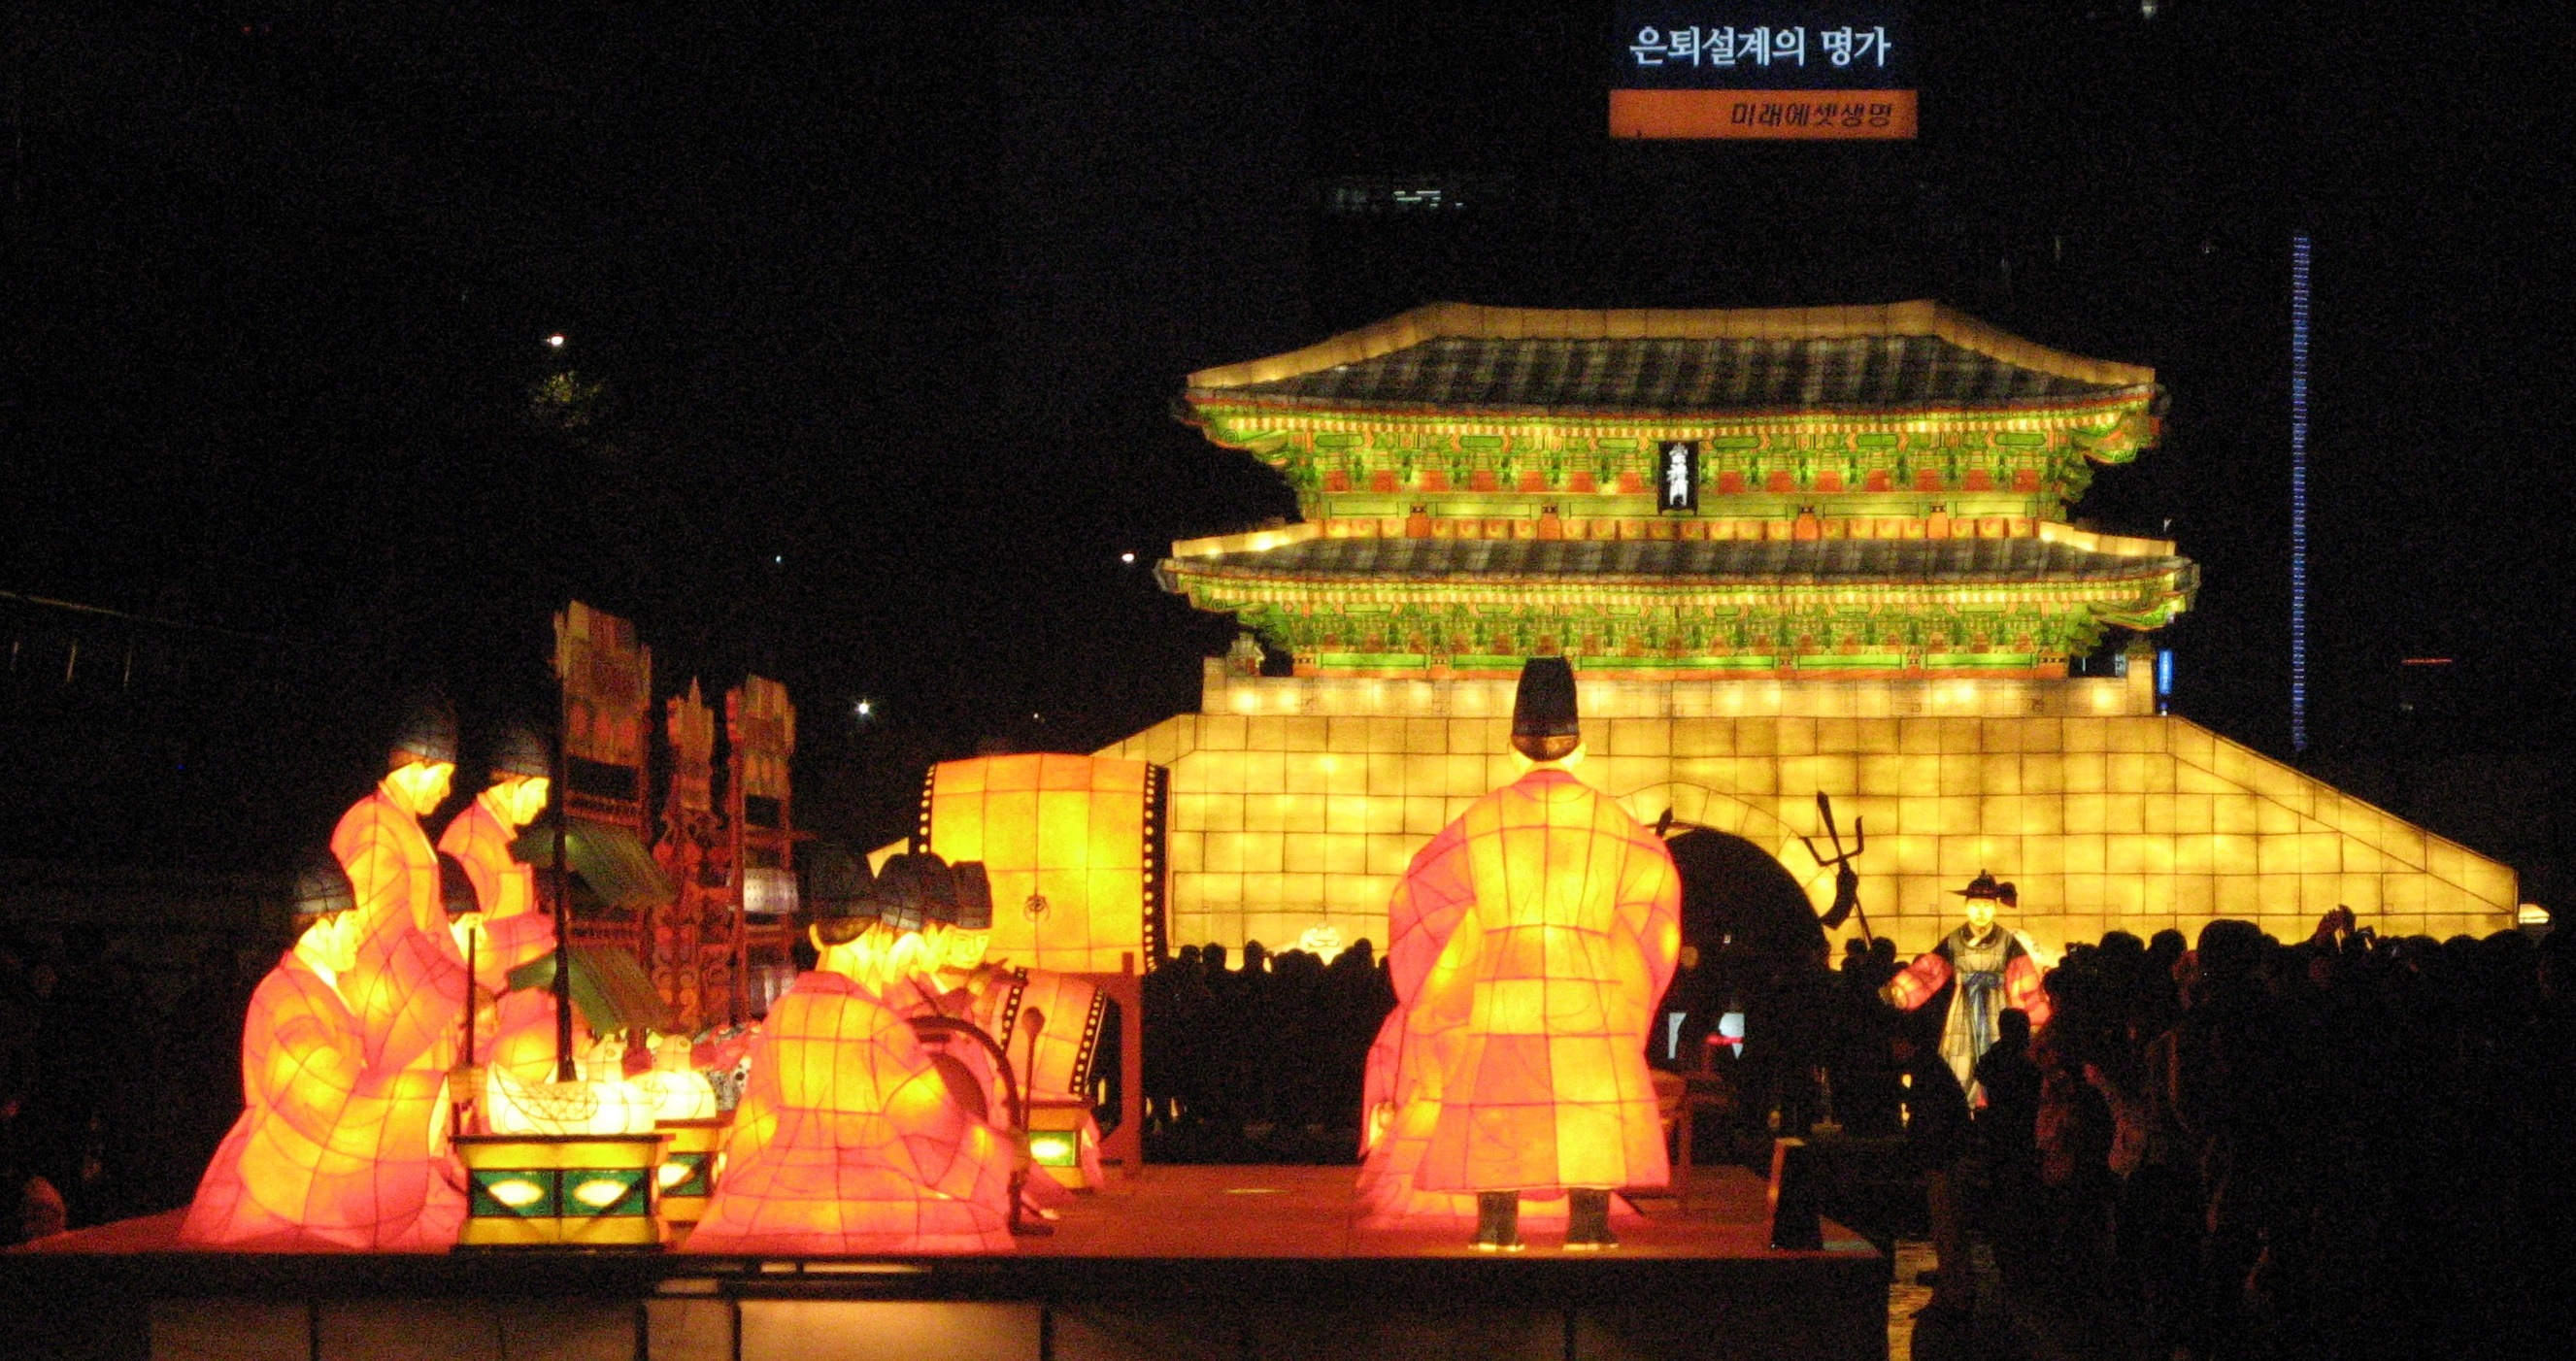
\includegraphics[height=9.7\baselineskip]{photos/11/23/img_2063.jpg}}
\vspace{-24pt}
\end{wrapfigure}The lanterns are located directly in the middle of the Cheong\-gye\-cheon stream, which is a small artificial creek with pathways on both sides. You were supposed to walk on the right side and return on the left one, which, surprisingly, worked out quite well. The ``statues'' were lighted using electric bulbs, as fire would be too unstable/dangerous/stupid. It was quite interesting to see all the electric cables in the water, but I guess they just had good insulation. Or insurance.

The whole exhibition was also some kind of contest, however, I am not sure about the rules or where the participants came from. The themes of the lanterns ranged from traditional Korean figures, over some Japanese figures, statues depicting child games, animals or abstract shapes to superheroes. Simply everything.

Approximately in the middle of the exhibition, there was a stand where you could buy your own lantern (real one with a candle) and put it in the stream. This surely looked romantic, unfortunately, these lanterns were stopped after few meters by a metal barrier, where they just kept piling up and setting themselves on fire. Not so romantic anymore.

\begin{figure}[h]
\centering
\subfigure{\fbox{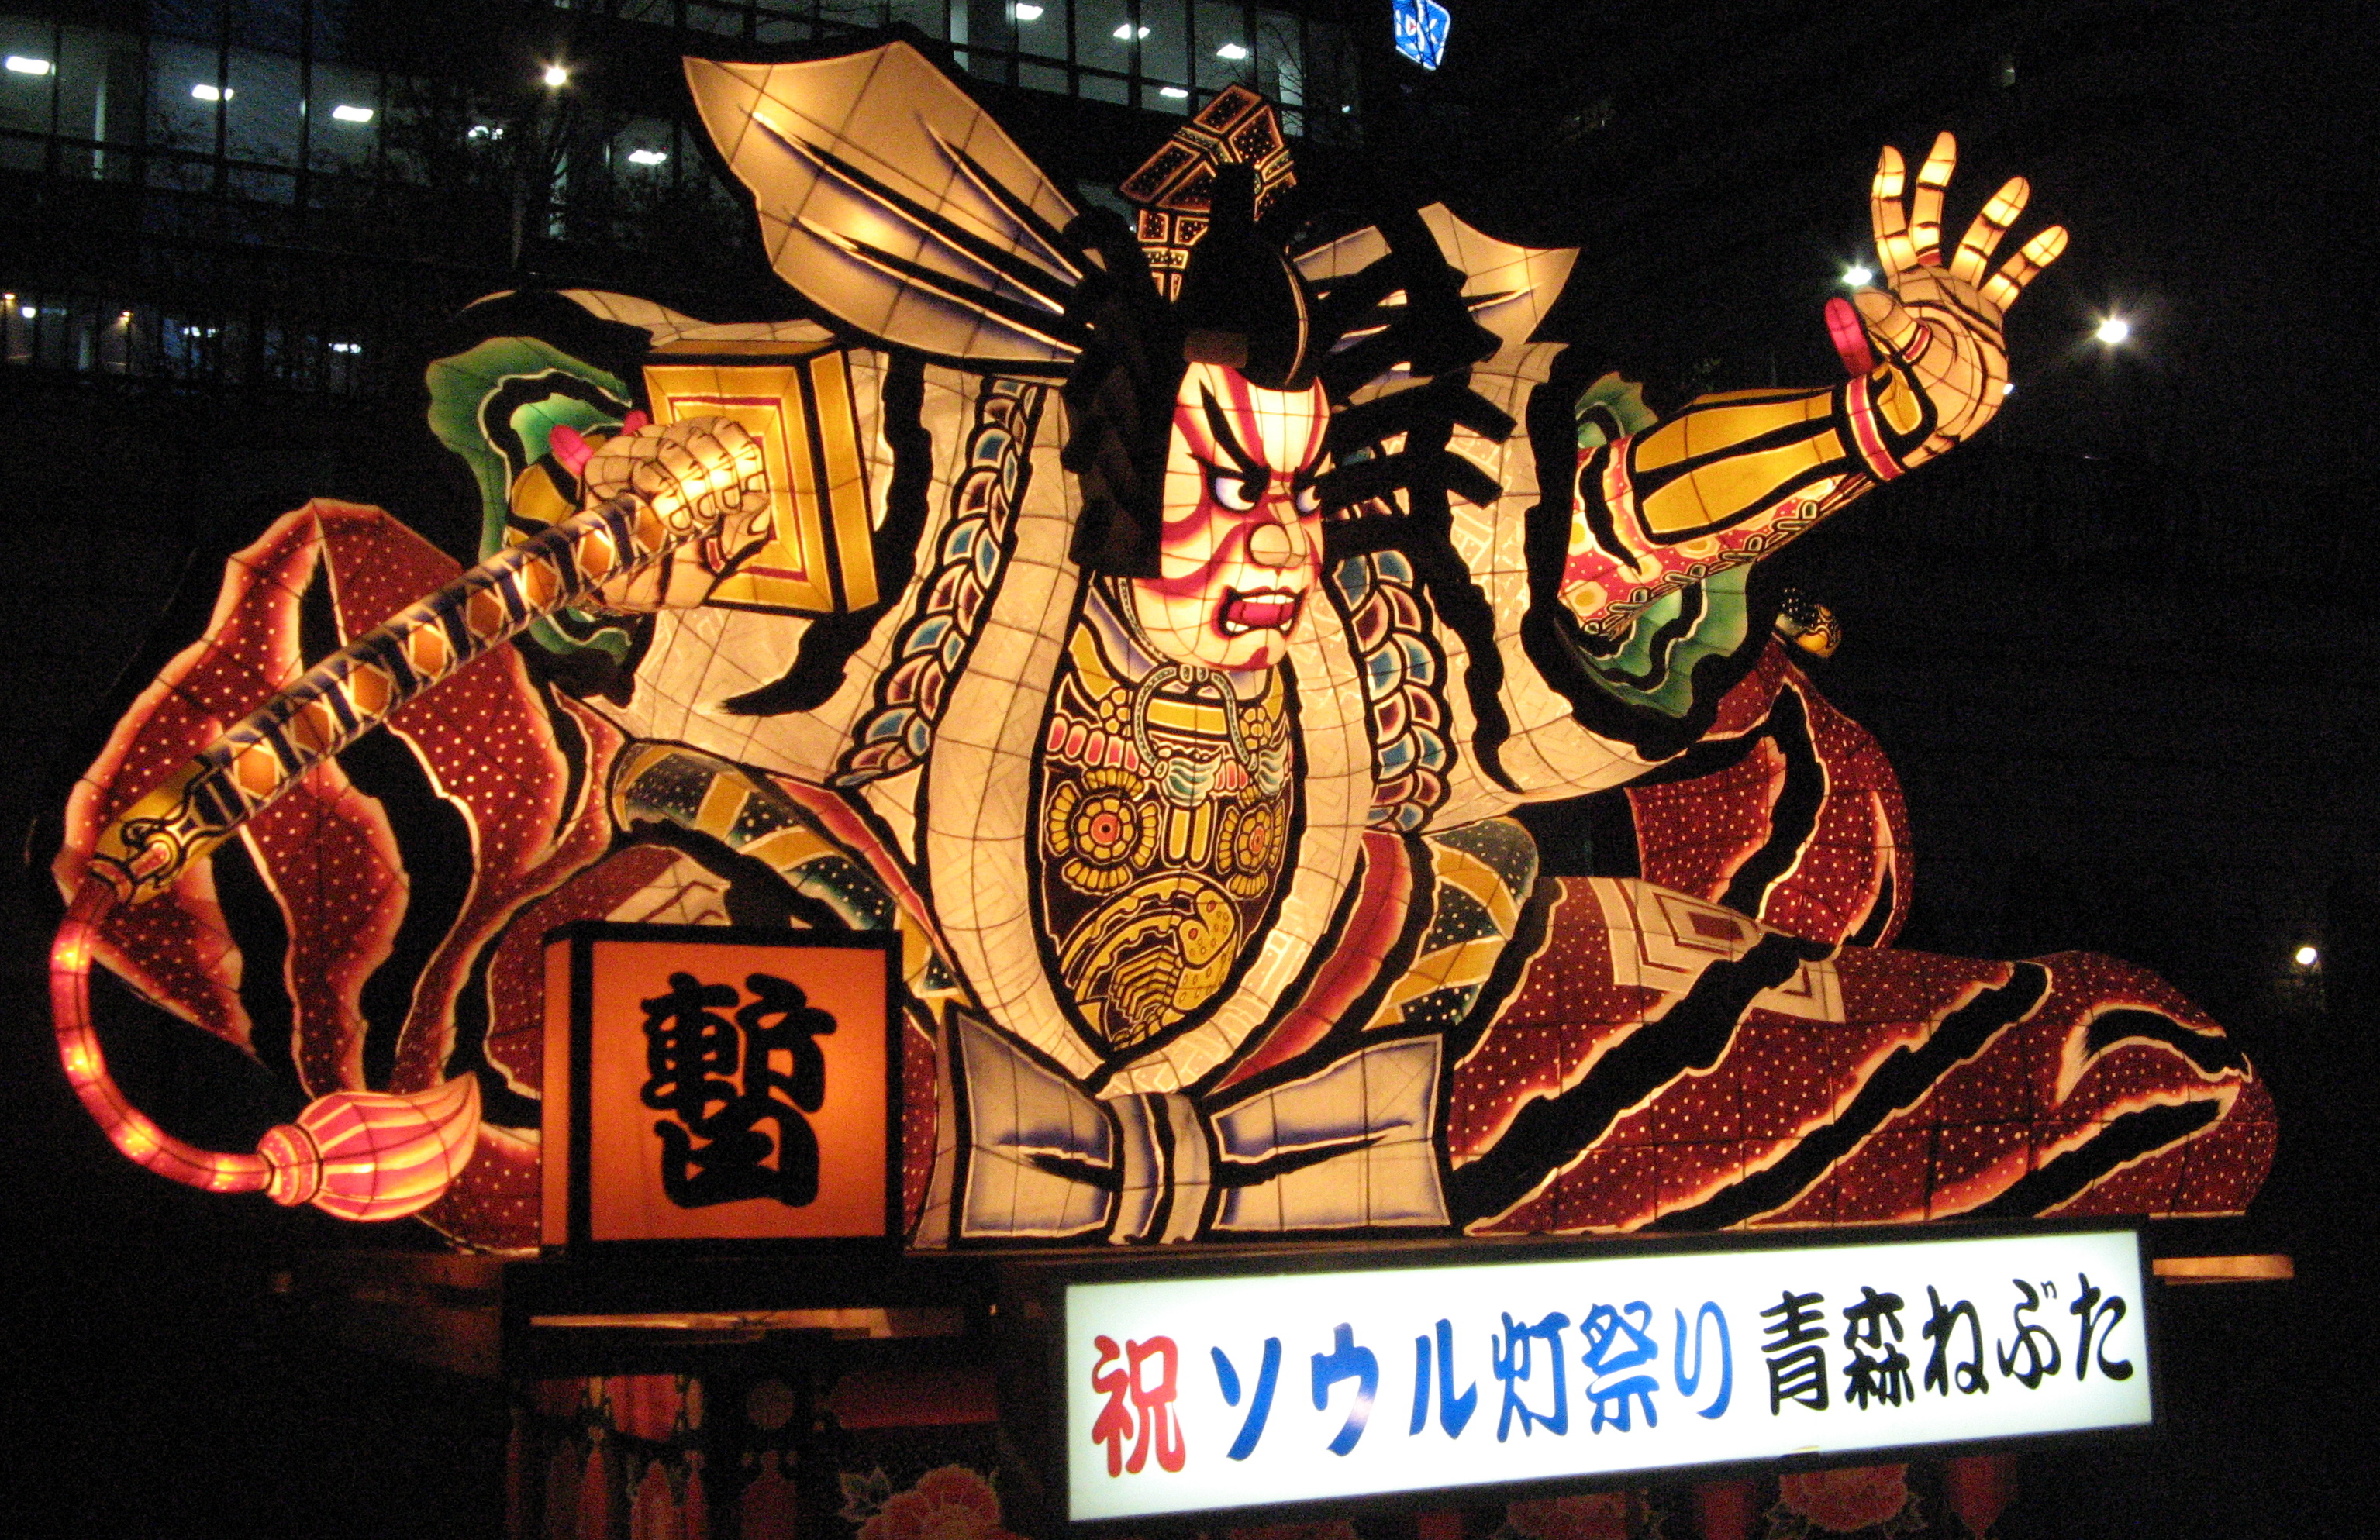
\includegraphics[height=0.28\textwidth]{photos/11/23/img_2107.jpg}}}
\subfigure{\fbox{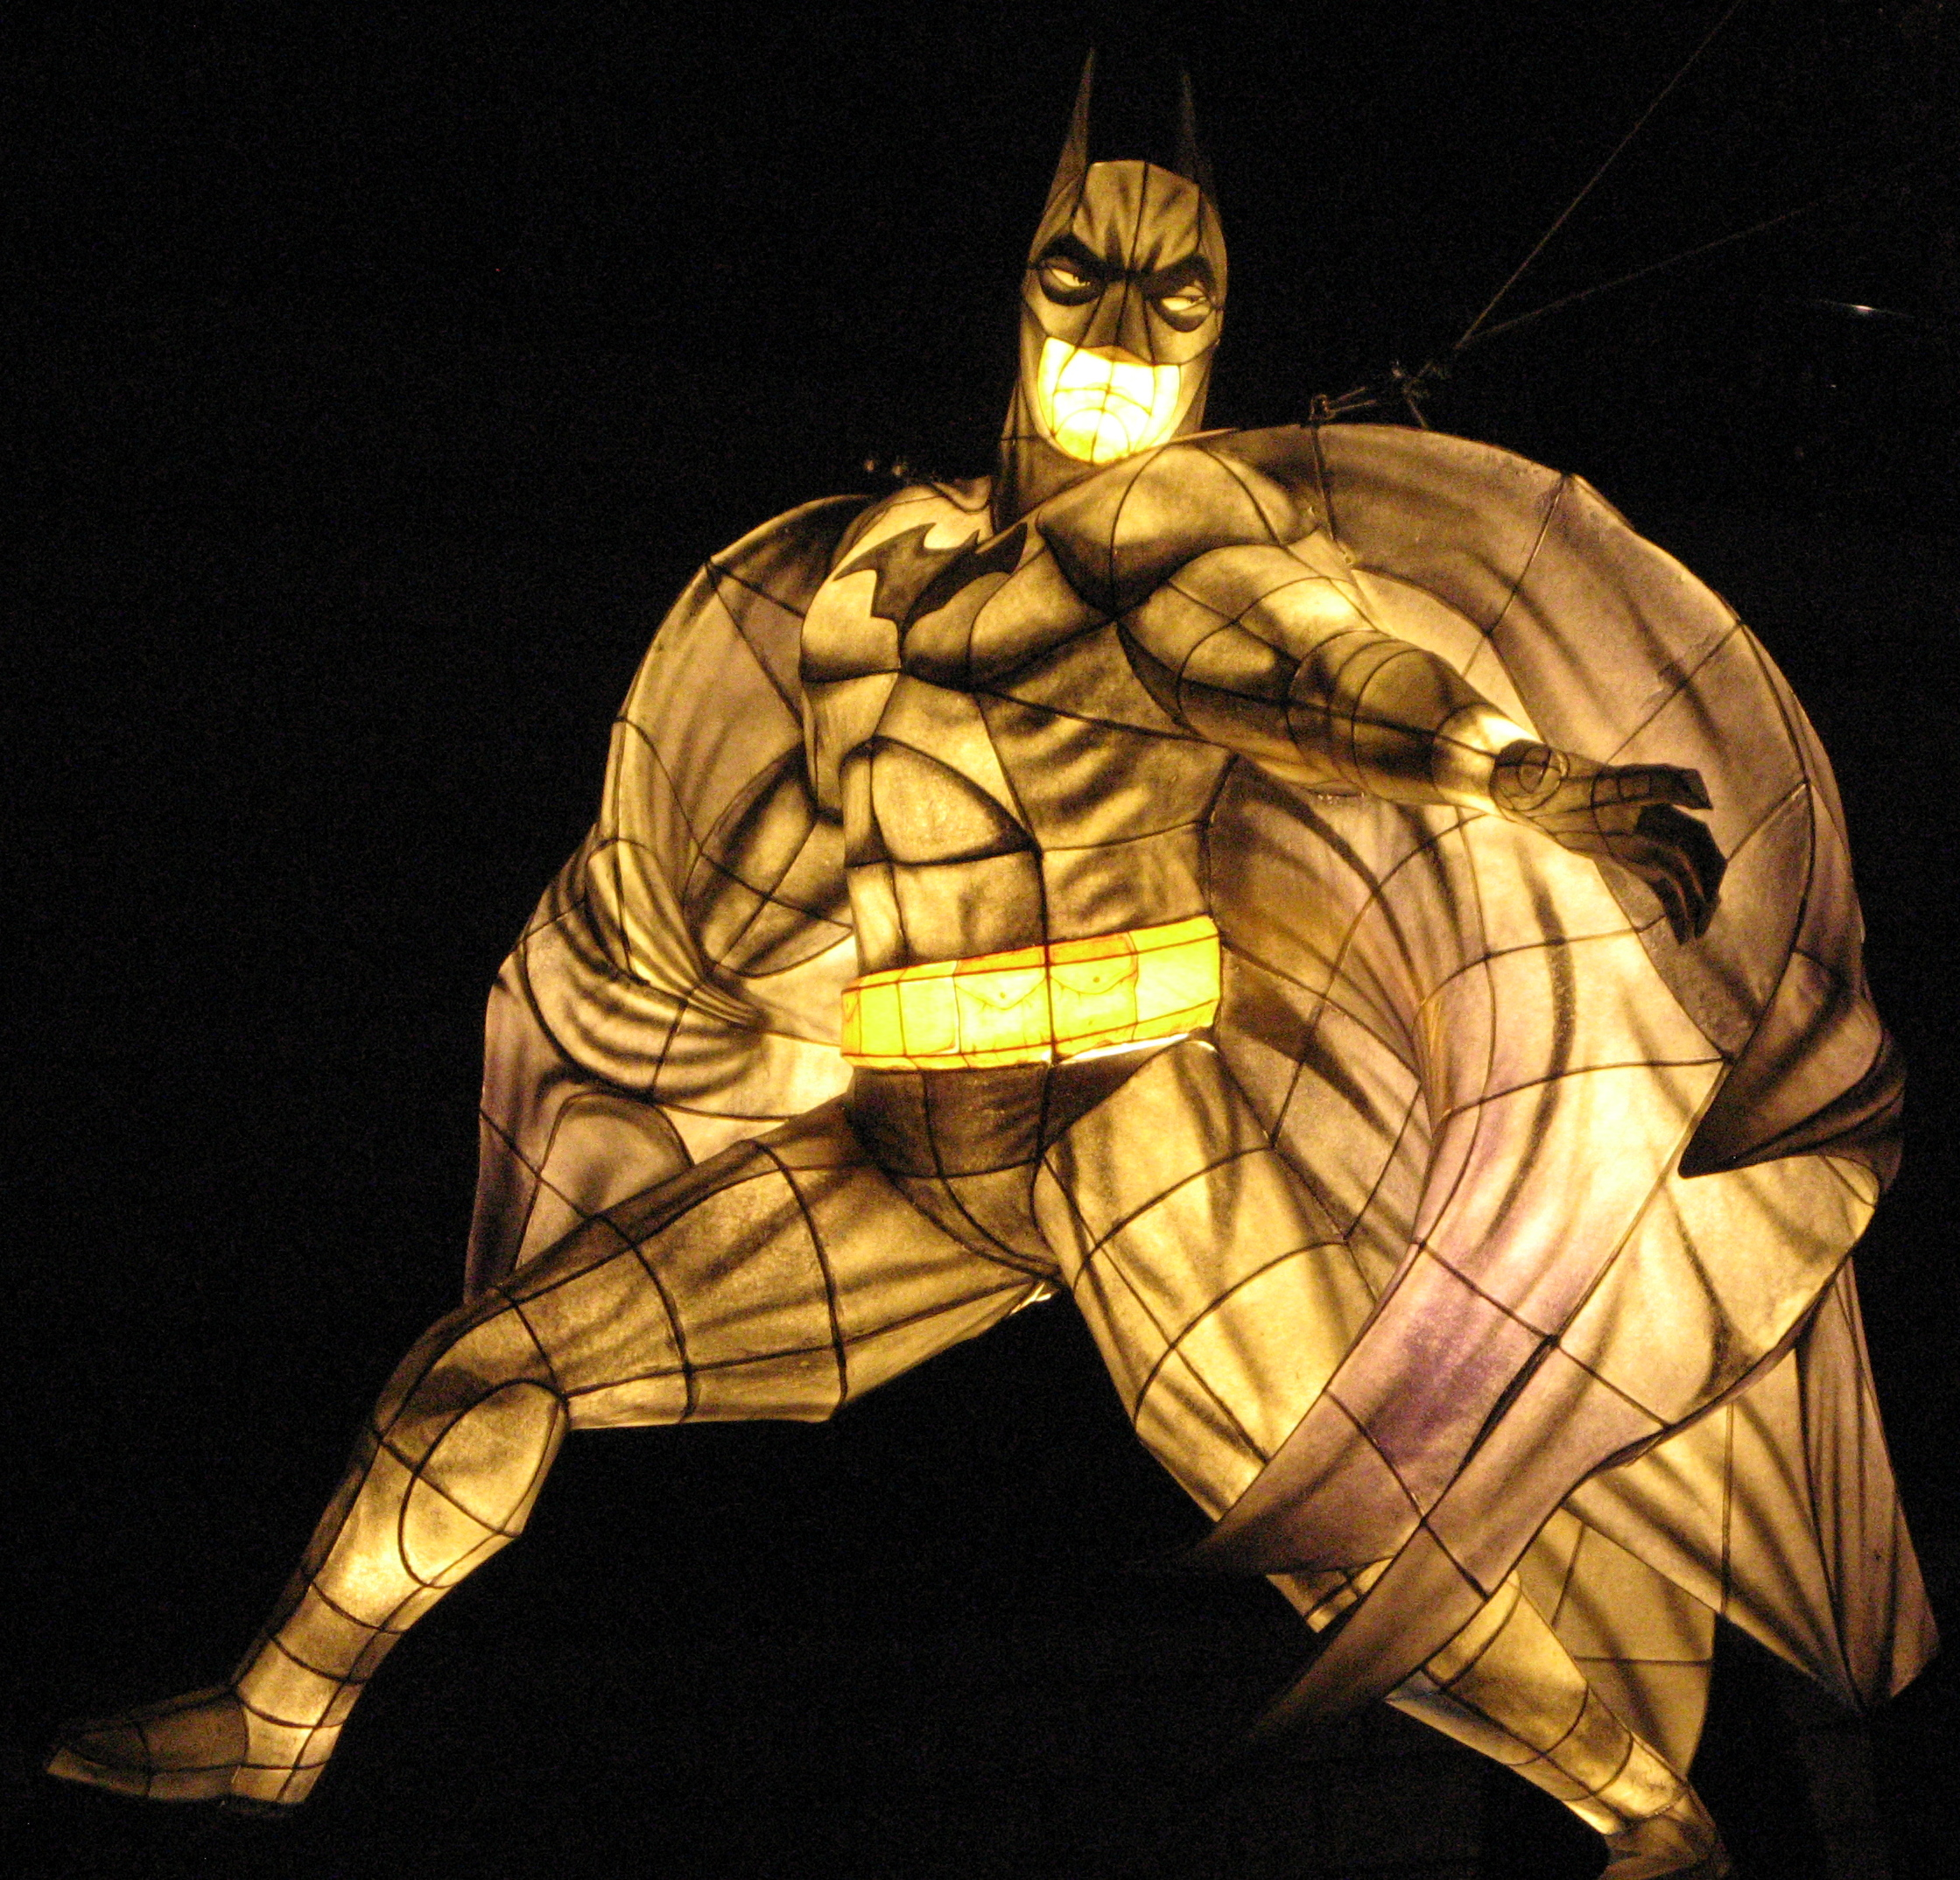
\includegraphics[height=0.28\textwidth]{photos/11/23/img_2098.jpg}}}
\end{figure}

The festival was really nice. Seeing all those colorful lanterns glow in the dark was amazing, especially in the combination with the creek. Since the creek is below ground level, I felt nicely isolated from the outer world, as well as the cold weather. The only bad thing about it was that we were not able to get any donuts afterwards. C'mon, people, 11pm is not too late for a donut, duh!
	\end{content}
\end{post}
